\pagenumbering{arabic}
\section{Mnist数据集}
\label{Ch:Mnist}
\subsection{关于Mnist数据集}
MNIST数据集作为机器学习界的“Hello World”,是学习模式识别和各大深度学习框架的基础数据库。2017年,
大神Hinton的最新研究方向CapsNet就是基于该数据集做的实验。该数据集是手写字符,如下图所示。
数据集源自NIST,后经CNN鼻祖Lecun等人修改后创建,共包含60000个训练样本和10000个测试样本,
验证样本每张图为28*28的灰度图像。
\begin{figure}[thbp!]
  \centering
  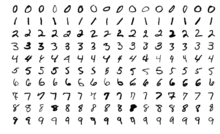
\includegraphics[width=0.4\linewidth]{figure/Ch0Mnist/220px-MnistExamples.png}
  \caption{MnistExamples}
  \label{fig:MnistExamples}
\end{figure}

\subsection{Mnist数据集组成}
训练数据集train和测试数据集test都分为label和image两个文件。image文件格式为idex3-ubyte,
label文件格式为idx1-ubyte。具体文件格式可以参见下图。像素灰度值为0-255,0代表白色,255代表黑色。
从图中可以看出训练集大小为60000,测试集大小为10000。每一幅图片大小为28*28。

\begin{figure}[htbp]
  \centering
  \begin{minipage}[t]{0.48\textwidth}
    \centering
    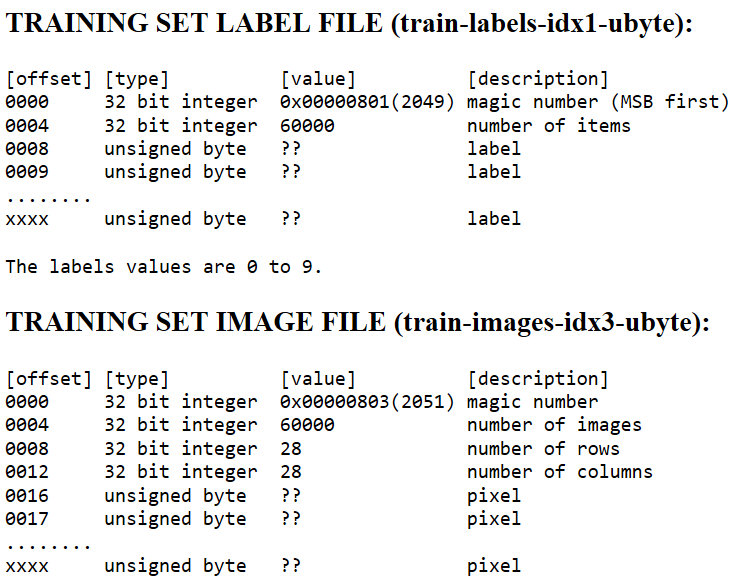
\includegraphics[width=6.5cm]{figure/Ch0Mnist/train.png}
    \caption{训练集image与label文件格式}
    \label{fig:ch0_train}
  \end{minipage}
  \begin{minipage}[t]{0.48\textwidth}
    \centering
    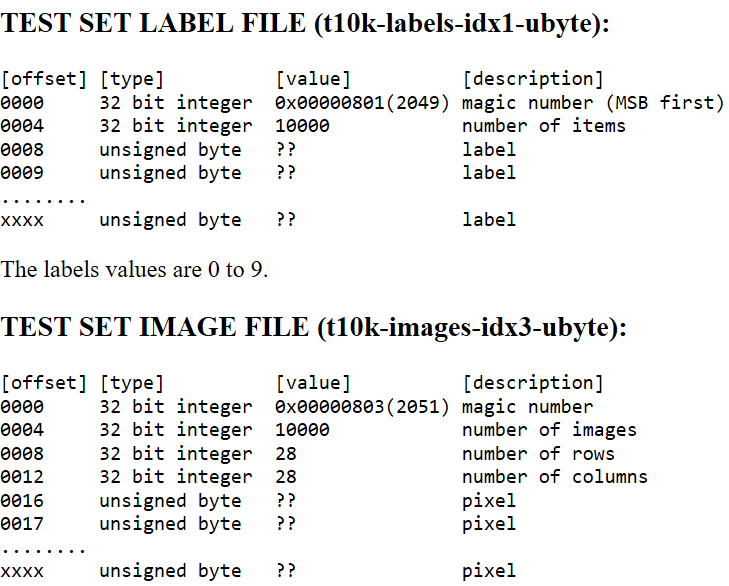
\includegraphics[width=6.5cm]{figure/Ch0Mnist/test.png}
    \caption{测试集image与label文件格式}
    \label{fig:ch0_test}
  \end{minipage}
\end{figure}

\subsection{Python中读取Mnist数据集}
读取mnist数据集其实就是读取二进制文件。
\subsubsection{idx3-ubyte文件解码}
\begin{python}
  def decode_idx3_ubyte(idx3_ubyte_file):
    # 读取二进制数据
    bin_data = open(idx3_ubyte_file, 'rb').read()

    # 解析文件头信息,依次为魔数、图片数量、每张图片高、每张图片宽
    offset = 0
    fmt_header = '>iiii' #因为数据结构中前4行的数据类型都是32位整型,所以采用i格式,但我们需要读取前4行数据,所以需要4个i。我们后面会看到标签集中,只使用2个ii。
    magic_number, num_images, num_rows, num_cols = struct.unpack_from(fmt_header, bin_data, offset)
    print('魔数:%d, 图片数量: %d张, 图片大小: %d*%d' % (magic_number, num_images, num_rows, num_cols))

    # 解析数据集
    image_size = num_rows * num_cols
    offset += struct.calcsize(fmt_header)  #获得数据在缓存中的指针位置,从前面介绍的数据结构可以看出,读取了前4行之后,指针位置(即偏移位置offset)指向0016。
    print(offset)
    fmt_image = '>' + str(image_size) + 'B'  #图像数据像素值的类型为unsigned char型,对应的format格式为B。这里还有加上图像大小784,是为了读取784个B格式数据,如果没有则只会读取一个值(即一副图像中的一个像素值)
    print(fmt_image,offset,struct.calcsize(fmt_image))
    images = np.empty((num_images, num_rows, num_cols))
    #plt.figure()
    for i in range(num_images):
        if (i + 1) % 10000 == 0:
            print('已解析 %d' % (i + 1) + '张')
            print(offset)
        images[i] = np.array(struct.unpack_from(fmt_image, bin_data, offset)).reshape((num_rows, num_cols))
        #print(images[i])
        offset += struct.calcsize(fmt_image)
#        plt.imshow(images[i],'gray')
#        plt.pause(0.00001)
#        plt.show()
    #plt.show()

    return images
\end{python}

\subsubsection{idx1-ubyte文件解码}
\begin{python}
  def decode_idx1_ubyte(idx1_ubyte_file):
    # 读取二进制数据
    bin_data = open(idx1_ubyte_file, 'rb').read()

    # 解析文件头信息,依次为魔数和标签数
    offset = 0
    fmt_header = '>ii'
    magic_number, num_images = struct.unpack_from(fmt_header, bin_data, offset)
    print('魔数:%d, 图片数量: %d张' % (magic_number, num_images))

    # 解析数据集
    offset += struct.calcsize(fmt_header)
    fmt_image = '>B'
    labels = np.empty(num_images)
    for i in range(num_images):
        if (i + 1) % 10000 == 0:
            print ('已解析 %d' % (i + 1) + '张')
        labels[i] = struct.unpack_from(fmt_image, bin_data, offset)[0]
        offset += struct.calcsize(fmt_image)
    return labels
\end{python}

\subsubsection{加载训练图片}
\begin{python}
  def load_train_images(idx_ubyte_file=train_images_idx3_ubyte_file):
    """
    TRAINING SET IMAGE FILE (train-images-idx3-ubyte):
    [offset] [type]          [value]          [description]
    0000     32 bit integer  0x00000803(2051) magic number
    0004     32 bit integer  60000            number of images
    0008     32 bit integer  28               number of rows
    0012     32 bit integer  28               number of columns
    0016     unsigned byte   ??               pixel
    0017     unsigned byte   ??               pixel
    ........
    xxxx     unsigned byte   ??               pixel
    Pixels are organized row-wise. Pixel values are 0 to 255. 0 means background (white), 255 means foreground (black).

    :param idx_ubyte_file: idx文件路径
    :return: n*row*col维np.array对象,n为图片数量
    """
    return decode_idx3_ubyte(idx_ubyte_file)
\end{python}

\subsubsection{加载训练标签}
\begin{python}
  def load_train_labels(idx_ubyte_file=train_labels_idx1_ubyte_file):
    """
    TRAINING SET LABEL FILE (train-labels-idx1-ubyte):
    [offset] [type]          [value]          [description]
    0000     32 bit integer  0x00000801(2049) magic number (MSB first)
    0004     32 bit integer  60000            number of items
    0008     unsigned byte   ??               label
    0009     unsigned byte   ??               label
    ........
    xxxx     unsigned byte   ??               label
    The labels values are 0 to 9.

    :param idx_ubyte_file: idx文件路径
    :return: n*1维np.array对象,n为图片数量
    """
    return decode_idx1_ubyte(idx_ubyte_file)
\end{python}

\subsubsection{加载测试图片}
\begin{python}
  def load_test_images(idx_ubyte_file=test_images_idx3_ubyte_file):
    """
    TEST SET IMAGE FILE (t10k-images-idx3-ubyte):
    [offset] [type]          [value]          [description]
    0000     32 bit integer  0x00000803(2051) magic number
    0004     32 bit integer  10000            number of images
    0008     32 bit integer  28               number of rows
    0012     32 bit integer  28               number of columns
    0016     unsigned byte   ??               pixel
    0017     unsigned byte   ??               pixel
    ........
    xxxx     unsigned byte   ??               pixel
    Pixels are organized row-wise. Pixel values are 0 to 255. 0 means background (white), 255 means foreground (black).

    :param idx_ubyte_file: idx文件路径
    :return: n*row*col维np.array对象,n为图片数量
    """
    return decode_idx3_ubyte(idx_ubyte_file)
\end{python}

\subsubsection{加载测试标签}
\begin{python}
  def load_test_labels(idx_ubyte_file=test_labels_idx1_ubyte_file):
    """
    TEST SET LABEL FILE (t10k-labels-idx1-ubyte):
    [offset] [type]          [value]          [description]
    0000     32 bit integer  0x00000801(2049) magic number (MSB first)
    0004     32 bit integer  10000            number of items
    0008     unsigned byte   ??               label
    0009     unsigned byte   ??               label
    ........
    xxxx     unsigned byte   ??               label
    The labels values are 0 to 9.

    :param idx_ubyte_file: idx文件路径
    :return: n*1维np.array对象,n为图片数量
    """
    return decode_idx1_ubyte(idx_ubyte_file)
\end{python}

\subsection{测试图片读取}
\begin{python}
  train_images = load_train_images()
  train_labels = load_train_labels()
  test_images = load_test_images()
  test_labels = load_test_labels()
  plt.figure(figsize=(10,10))
  for i in range(9):
      plt.subplot(3,3,i+1)
      plt.imshow(train_images[i], cmap='gray')
      plt.title("label: "+str(int(train_labels[i])))
  plt.show()
\end{python}
输出如图\ref{fig:ch0loaddatatest}所示:
\begin{figure}[thbp!]
  \centering
  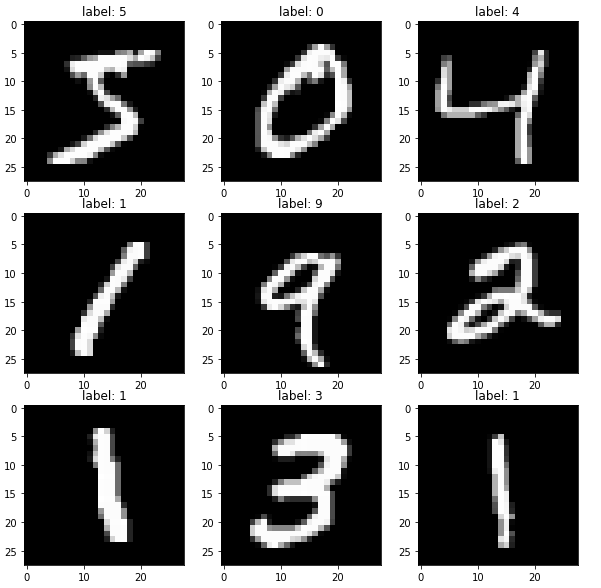
\includegraphics[width=0.3\linewidth]{figure/Ch0Mnist/loaddatatest.png}
  \caption{测试数据读取}
  \label{fig:ch0loaddatatest}
\end{figure}






